% !TEX encoding = UTF-8
% !TEX program = pdflatex
% !TEX root = InformationRetrieval.tex
% !TEX spellcheck = it-IT

% 11 Novembre 2016
%\chapter{Sistemi di reperimento dell'informazione}
%\section{Configurazione di Terrier per il nostro progetto}
\chapter{Valutazione dei sistemi di reperimento}

\section{Cosa vuol dire valutare un IRS}

Un sistema di reperimento può essere valutato per vari motivi, tipicamente perché è necessario rispondere alle domande:

\begin{itemize}
	\item quale motore di ricerca è preferibile utilizzare per le proprie ricerche?
	\item quale sistema conviene utilizzare all'interno di un motore di ricerca?
	\item quale sistema commerciale conviene acquistare?
	\item come posso migliorare l'interfaccia utente?
\end{itemize}

\noindent Il tutto si può riassumere in un ``valutiamo per capire come migliorare il nostro sistema''. Bisogna quindi essere in grado di capire come effettivamente opera un IRS e di prendere decisioni utili.

Pertanto la valutazione di un IRS si basa sull'efficacia del sistema, misurando quanto bene un sistema IR si comporta nel reperire documenti di interesse per una specifica utenza.
Servono quindi dei test scientifici che permettano di capire come il sistema si comporta a seconda delle diverse situazioni di reperimento dell'informazione in cui potrebbe essere utilizzato. Per garantire la ripetibilità dell'esperimento è necessario basarsi su delle collezioni di test.

\section{Le basi della valutazione}

L'approccio \textbf{Cranfield} è uno standard per la valutazione dei sistemi IR.
\`E stato inventato dal bibliotecario del college di Cranfield e da un groppo di persone che lavoravano con lui, senza l'utilizzo di computer, siamo nel 1958. 
Sono stati elaborati due test:

\subsection{Cranfield 1} 

Si voleva testare il funzionamento di 4 diversi metodi di indicizzazione manuale. Ci sono dei bibliotecari esperti che classificano manualmente i vari libri in modo che gli utenti possano ricercare agevolmente i libri riguardanti un determinato argomento.

All'epoca l'unico modo di accesso all'informazione era manuale e avveniva mediante degli indici suddivisi per argomento e creati dai bibliotecari.
La proposta di Cranfield 1 contiene 18.000 articoli e rapporti da indicizzare, secondo 4 criteri di indicizzazione (per soggetto, a faccette, Classificazione Decimale Universale, Coordinate and Unitrem Index Systems). L'indicizzazione doveva essere fatta da delle persone competenti ed in modo sistematico.
	
All'epoca però non c'era il concetto di reperimento, quindi ad un'interrogazione bastava recuperare uno documento che di sicuro era rilevante per la domanda (\textbf{known item searching}). Le domande venivano pensate dagli autori dei documenti che erano indicizzati, in questo modo si sapeva già quali dovevano essere le risposte.
	
Del processo di ricerca manuale sull'indice è stata tenuta traccia del tempo per effettuare la ricerca e dell'esito della ricerca. Dall'esperimento effettuato, il 35\% delle ricerche non è andata a buon fine e non ha dimostrato una differenza tra i 4 sistemi.
Parte di questo risultato è però dovuto ad errori degli indicizzatori.
	
Dai risultati l'esperimento sembra mal riuscito ma ha fatto emergere la \textbf{failure analysis}, ovvero la documentazione dei fallimenti e l'utilizzo di questa per evitare di fare altri errori simili. Le considerazioni erano riguardanti anche il formato dei descrittori, la quantità, se questi portavano a uno o più risultati e sull'assenza dei pesi per i descrittori.
	
\subsection{Cranfield 2}

Questo test riduce il numero di documenti ed effettua una costruzione preliminare della collezione dei documenti. I documenti dovevano essere scelti in modo che fossero un campione rappresentativo della realtà. Durante questa fase dovevano essere anche preparate le domande, prima di aver letto i documenti, perché l'utente normale tipicamente non ne conosce il contenuto quando formula la query.

Per indicizzare la collezione sono stati utilizzati tutti i 33 metodi noti, che sono stati poi valutati secondo delle \textbf{metriche di valutazione}.

Le metriche utilizzate sono note come \textbf{Precision} e \textbf{Recall} e vengono rappresentate in una \textbf{tabella di contingenza}.

% inserimento della tabella di contingenza slide 20

\noindent \textbf{Recall} rappresenta il rapporto tra i documenti rilevanti che recuperiamo in risposta ad un'interrogazione e tutti i documenti rilevanti della collezione. Ovviamente più vicino a 1 è meglio.

$$
recall = \frac{a}{a+c}
$$

\noindent \textbf{Precision} rappresenta il rapporto tra i documenti rilevanti che sono stati recuperati e tutti i documenti che sono presenti nella collezione. Anche qui, più vicino a 1 è meglio.

$$
precision = \frac{a}{a+b}
$$

Nell'esperimento di Cranfield, queste misure sono state calcolate tutte le 221 domande (\textbf{run}).
Ci fu quindi il problema di combinare i risultati ottenuti. Questo è stato fatto con il \textbf{micro-averaging method}: vengono fatte le somme totali dei numeri dei rilevati e dei recuperati di tutte le domante e poi sono state divisi per il numero di domande.

Dai risultati riporta in figura \ref{l13:fig1} è emerso che i sistemi di indicizzazione migliori erano quelli che utilizzavano i singoli termini presi dai vari documenti. Quindi era meglio utilizzare i termini dei documenti piuttosto che delle combinazioni fittizie create a priori (\textbf{Paradigma Cranfield}). 

\begin{figure}
	\centering
	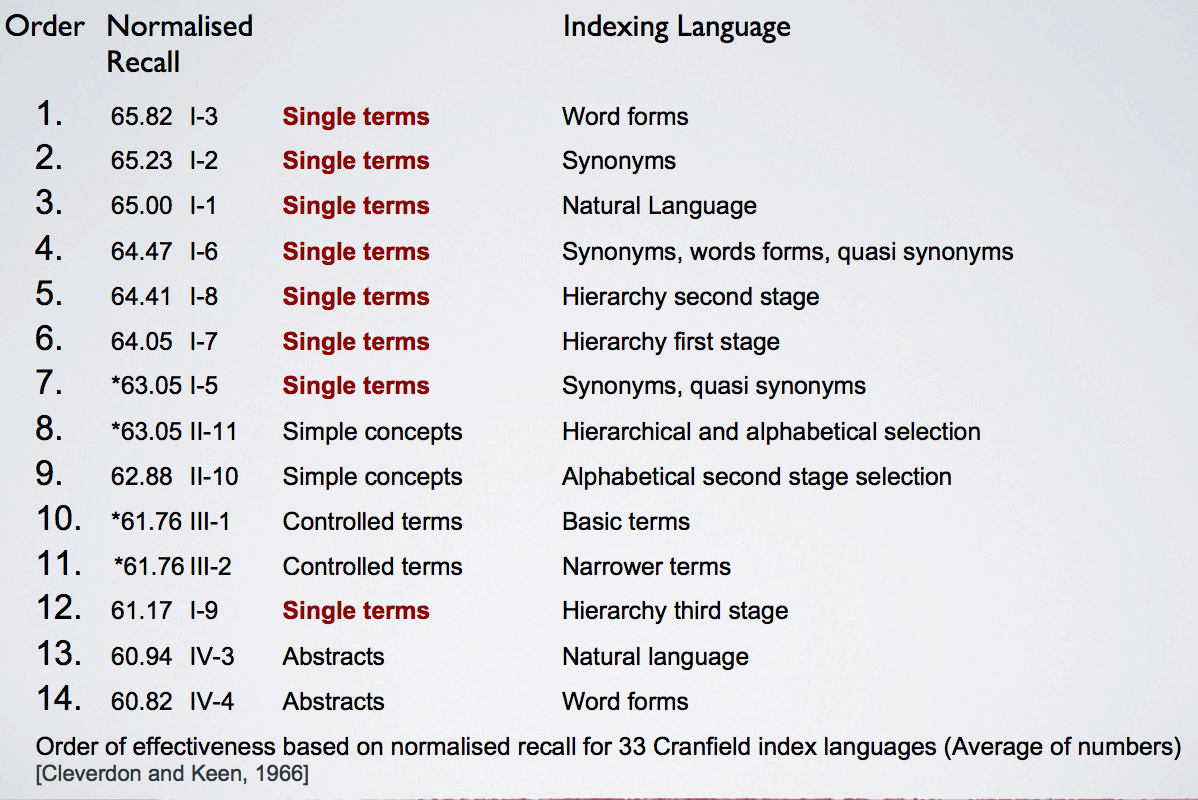
\includegraphics[width=.6\textwidth]{images/l13-fig-1.png}
	\label{l13:fig1}
\end{figure}

\subsection{Il sistema SMART}

Nel 1961 ad Harvard hanno il primo sistema automatico di reperimento dell'informazione SMART ad opera di Gerald Salton.

Gli esperimenti eseguiti con SMART producevano liste ordinate o semi-ordinate e pertanto non era possibile utilizzare precision e recall. 
Sono state quindi proposte nuove metriche come \textbf{rank recall}, \textbf{log precision}, \textbf{normalized recall} e \textbf{normalized precision}. Queste metriche sono più complesse perché prendono in vengono calcolati sui primi \textit{N} risultati. 

\section{Il paradgima Cranfield}

In linea di massima si tratta di effettuare una simulazione utente/task.

Cleverdon ha modellato il \textbf{task di ricerca} di un insieme di documenti costruendo una collezione di test da usare ripetutamente in diversi esperimenti di laboratorio invece di eseguire uno studio d'utente diverso per ogni metodo di indicizzazione da valutare.
Serve quindi una collezione coerente con il task di ricerca d'interesse.

Questo metodo permette di riusare una collezione di test per molti esperimenti, permettendoci di \textbf{ripeterli} e di crearne di nuovi che prima non erano stati immaginati alla creazione della collezione.

La modellazione del task di ricerca è molto importante e deve essere definito a priori, come l'intento di recuperare un singolo documento rilevante (\textbf{known-item search}) oppure tutti i documenti rilevanti.

Alcuni esempi sono delle ricerche ad-hoc su una collezione di documenti su uno specifico argomento (es: articoli finanziari), oppure delle ricerche rispetto ad un argomento specifico (es: brevetti) o su documenti multimediali.

Per definire un test è quindi necessario specificare il \textbf{corpus di documenti} pertinenti al task, l'insieme di domande alle quali si vuole rispondere (\textbf{topic}) e i \textbf{giudizi di rilevanza}, in modo che sia possibile dire se un documento è rilevante o meno rispetto ad un dato topic.

Tutto questo prende il nome di \textbf{collezione sperimetnale di reperimento dell'informazione} o \textbf{test collection}, ed è una tripla:

$$
C = \langle D, T, RJ\rangle
$$

\noindent dove:
\begin{itemize}
	\item $C$ è la collezione sperimentale di test
	\item $D$ è l'insieme dei documenti
	\item $T$ è l'insieme dei topic
	\item $RJ$ è l'insieme dei giudizi di rilevanza
\end{itemize}

\noindent Le metriche che possono essere utilizzate sono precision e recall, ma anche altre più complesse.

Creare una collezione di test è un lavoro molto oneroso in termini di tempo e di risorse umane, pertanto tipicamente vengono utilizzate delle collezioni pubbliche.

La prima collezione sperimentale pubblica è CACM nel 1982, contenente tutti i titoli e abstract degli articoli scentifici delle CACM dal 1958 e 1979. I topics sono le interrogazioni reali effettuate dagli utenti (professori e studenti di informatica) di diverse biblioteche americane e i giudizi di rilevanza sono stati dati da questi utenti ma solo su documenti che avevano un'alta probabilità di essere rilevanti.













